\documentclass[12pt,a4paper]{article}

% --------------------------------------------------
% Pacotes
% --------------------------------------------------
\usepackage[T1]{fontenc}
\usepackage[utf8]{inputenc}
\usepackage[main=brazil]{babel}

\usepackage[
    a4paper,
    margin=2.5cm,
    top=3.2cm,
    headheight=70pt,
    headsep=18pt
]{geometry}
\usepackage{graphicx}

\usepackage{amsmath,amssymb}
\usepackage{caption}
\usepackage{setspace}
\usepackage{titlesec}
\usepackage{indentfirst}
\usepackage{float}
\usepackage{newtxtext,newtxmath}
\usepackage[hidelinks]{hyperref}
\usepackage{fancyhdr}

% --------------------------------------------------
% Cabeçalho
% --------------------------------------------------
\pagestyle{fancy}
\fancyhf{}
\fancyhead[R]{
\includegraphics[height=1.8cm]{base_images/logo-puc.png}}
\renewcommand{\headrulewidth}{0pt}

% --------------------------------------------------
% Ajustes visuais
% --------------------------------------------------
\setlength{\parindent}{1.25cm}
\setlength{\parskip}{0pt}
\onehalfspacing

\captionsetup{
    font=small,
    labelfont=normalfont,
    justification=centering
}

\titleformat{\subsection}
  {\normalfont\bfseries\large}
  {\thesubsection}
  {0.6em}
  {}

% --------------------------------------------------
% Comandos úteis
% --------------------------------------------------
\newcommand{\question}[1]{
    \vspace{0.8em}
    \noindent\textit{#1}
    \vspace{0.4em}
}

\newcommand{\answer}{
    \par
}

% --------------------------------------------------
% Documento
% --------------------------------------------------
\begin{document}

% Título
\begin{center}
    {\LARGE \textbf{ENG4448 - Laboratório de Computação Digital}}\\[0.3cm]
    {\Large Relatório do Laboratório 07}\\[0.2cm]
    27/05/2026 - Rio de Janeiro
\end{center}

\vspace{0.8cm}

% Informações da dupla
\noindent \textbf{Turma 3VA - Dupla:}\\
Pedro Coelho Carneiro da Cunha - 2310837\\
Pedro Carneiro Nogueira - 2310540

\vspace{0.5cm}
\hrule
\vspace{0.8cm}

\setcounter{section}{1}
\setcounter{subsection}{0}

\section{Roteiro}

% ==============================================================
\subsection{Exercício 1 – Display LCD: Inicialização}
% ==============================================================

\question{Implemente os módulos VHDL para controlar o display LCD, incluindo a sequência
de inicialização em modo 4 bits, a configuração do controlador e a escrita de uma mensagem
de ao menos três palavras.}

\answer
A implementação foi organizada em quatro arquivos VHDL: um pacote de utilitários
(\texttt{lcd\_utils\_pkg.vhd}) e três módulos hierárquicos, módulo de inicialização
(\texttt{lcd\_init.vhd}), módulo de escrita (\texttt{lcd\_write.vhd}) e módulo de topo
(\texttt{top.vhd}). O display LCD opera em modo de 4 bits na placa: cada byte é transmitido em dois \textit{nibbles} (meios bytes)
consecutivos pelo barramento compartilhado \texttt{SF\_D[11:8]}.

\subsubsection{Pacote de Utilitários (\texttt{lcd\_utils\_pkg.vhd})}

O pacote centraliza as definições reutilizadas por todos os módulos:

\begin{itemize}
    \item \textbf{Tipos}: \texttt{byte\_t} (8 bits), \texttt{nibble\_t} (4 bits),
          \texttt{char\_array\_type} (arranjo de 16 bytes, para linhas de texto) e
          \texttt{initcmd\_array\_type} (arranjo de 4 bytes, para comandos de configuração).
    \item \textbf{Constantes de temporização} (Tabela~\ref{tab:timing}): expressas em
          número de ciclos para o clock de 50\,MHz da placa (período de 20\,ns).
    \item \textbf{Procedimento \texttt{increment\_and\_check}}: a cada chamada, incrementa
          um contador de 20 bits; quando este atinge o valor \textit{limite}$-1$, zera o
          contador e sinaliza (variável booleana \texttt{is\_done} $\leftarrow$ \texttt{true})
          que o tempo expirou. Esse procedimento é invocado nos processos síncronos para
          implementar todas as esperas temporizadas.
\end{itemize}

\begin{table}[H]
\centering
\begin{tabular}{lrr}
\hline
\textbf{Constante} & \textbf{Ciclos} & \textbf{Tempo} \\
\hline
\texttt{wait750k} & 750\,000 & 15{,}0\,ms \\
\texttt{wait205k} & 205\,000 &  4{,}1\,ms \\
\texttt{wait82k}  &  82\,000 &  1{,}64\,ms \\
\texttt{wait5k}   &   5\,000 & 100\,$\mu$s \\
\texttt{wait2k}   &   2\,000 &  40\,$\mu$s \\
\texttt{wait50}   &      50  &   1\,$\mu$s \\
\texttt{wait12}   &      12  & 240\,ns \\
\texttt{wait2}    &       2  &  40\,ns \\
\hline
\end{tabular}
\caption{Constantes de temporização definidas em \texttt{lcd\_utils\_pkg.vhd}
         (clock de 50\,MHz).}
\label{tab:timing}
\end{table}

\subsubsection{Módulo de Inicialização (\texttt{lcd\_init.vhd})}

O módulo implementa a sequência de inicialização em modo 4 bits do controlador do LCD
por meio de uma máquina de estados finitos (FSM) com 13 estados
(\texttt{STEP0}–\texttt{STEP8} e \texttt{DONE}). A sequência, resumida na
Tabela~\ref{tab:init_seq}, garante que o display parta de um estado conhecido logo após
a energização.

\begin{table}[H]
\centering
\begin{tabular}{cccr}
\hline
\textbf{Passo} & \textbf{Dado} & \textbf{Enable} & \textbf{Ciclos @ 50\,MHz} \\
\hline
0 & ---  & 0 & 750\,000 \\
1 & 0x3  & 1 & 12 \\
2 & ---  & 0 & 205\,000 \\
3 & 0x3  & 1 & 12 \\
4 & ---  & 0 & 5\,000 \\
5 & 0x3  & 1 & 12 \\
6 & ---  & 0 & 2\,000 \\
7 & 0x2  & 1 & 12 \\
8 & ---  & 0 & 2\,000 \\
\hline
\end{tabular}
\caption{Sequência de inicialização implementada em \texttt{lcd\_init.vhd}.}
\label{tab:init_seq}
\end{table}

O passo 0 aguarda 15\,ms após a liberação do reset, garantindo a estabilização da
alimentação. Os três primeiros pulsos de \textit{enable} (passos 1, 3 e 5) enviam o
nibble \texttt{0x3} com \texttt{LCD\_RS = 0} e \texttt{LCD\_RW = 0}, forçando o
controlador a executar um \textit{Function Set} em modo de 8 bits, necessário para
levar o display a um estado determinístico, independentemente de como ele foi
inicializado. O quarto pulso (passo 7) envia \texttt{0x2}, instruindo o controlador a
alternar definitivamente para o modo de 4 bits. Ao término do passo 8 (espera de
40\,$\mu$s), o sinal \texttt{LCD\_INIT\_DONE} é levado a '1', notificando o módulo de
escrita que o display está pronto.

Cada estado de \textit{enable} é subdividido em dois subestados: um de \textit{setup}
(2 ciclos com \texttt{LCD\_E = '0'} enquanto o dado se estabiliza) e um com
\texttt{LCD\_E = '1'} (12 ciclos, equivalentes a 240\,ns de pulso ativo).

\subsubsection{Módulo de Escrita (\texttt{lcd\_write.vhd})}

O módulo aguarda \texttt{LCD\_INIT\_DONE = '1'} para começar a operar e é estruturado
em duas FMSs hierárquicas: uma \textit{FMS mestre} que controla o fluxo de alto nível e
uma \textit{FMS de escrita} que gerencia a transmissão byte a byte.

\paragraph{FMS Mestre (\texttt{master\_fsm}).}
Percorre os seguintes estados em sequência:

\begin{enumerate}
    \item \textbf{SEND\_CONFIG}: envia os quatro comandos de configuração da
          Tabela~\ref{tab:config_cmds} com \texttt{LCD\_RS = 0} (modo comando).
    \item \textbf{SEND\_LINE1}: escreve os 16 caracteres da primeira linha com
          \texttt{LCD\_RS = 1} (modo dado).
    \item \textbf{LINE\_CHANGE}: envia o comando \texttt{0xC0}
          (\textit{Set DDRAM Address} para o endereço 0x40, início da segunda linha).
    \item \textbf{SEND\_LINE2}: escreve os 16 caracteres da segunda linha.
    \item \textbf{DONE}: permanece ocioso; escrita concluída.
\end{enumerate}

\begin{table}[H]
\centering
\begin{tabular}{clr}
\hline
\textbf{Comando} & \textbf{Descrição} & \textbf{Espera pós-envio} \\
\hline
\texttt{0x28} & \textit{Function Set}: modo 4 bits, 2 linhas, 5$\times$8 dots & 40\,$\mu$s \\
\texttt{0x06} & \textit{Entry Mode Set}: incremento automático do cursor       & 40\,$\mu$s \\
\texttt{0x0F} & \textit{Display On/Off}: display, cursor ligados e piscando    & 40\,$\mu$s \\
\texttt{0x01} & \textit{Clear Display}                                          & 1{,}64\,ms \\
\hline
\end{tabular}
\caption{Comandos de configuração enviados após a inicialização.}
\label{tab:config_cmds}
\end{table}

\paragraph{FMS de Escrita (\texttt{write\_fsm}).}
Para cada byte, a FMS percorre os estados abaixo, respeitando a temporização da
interface de 4 bits:

\begin{enumerate}
    \item \textbf{UPPER\_NIBBLE}: posiciona \texttt{DATA\_OUT[7:4]} no barramento e
          aguarda 2 ciclos (\textit{setup}).
    \item \textbf{UPPER\_NIBBLE\_E}: ativa \texttt{LCD\_E = '1'} por 12 ciclos
          (240\,ns).
    \item \textbf{WAIT\_1U}: desativa \texttt{LCD\_E} e aguarda 50 ciclos
          (1\,$\mu$s) entre os dois nibbles.
    \item \textbf{LOWER\_NIBBLE}: posiciona \texttt{DATA\_OUT[3:0]} e aguarda 2 ciclos.
    \item \textbf{LOWER\_NIBBLE\_E}: ativa \texttt{LCD\_E = '1'} por 12 ciclos.
    \item \textbf{WAIT\_POST\_BYTE}: desativa \texttt{LCD\_E} e aguarda 2\,000 ciclos
          (40\,$\mu$s) entre bytes comuns, ou 82\,000 ciclos (1{,}64\,ms) após o
          \textit{Clear Display}.
\end{enumerate}

\paragraph{Mensagem exibida.}
O grupo escolheu a frase \textit{``Durma bem cedo, OK?''}, distribuída nas duas linhas
do display LCD:

\begin{itemize}
    \item \textbf{Linha 1}: \texttt{"Durma bem       "} — caracteres ASCII nas
          posições 0–8 do arranjo \texttt{FIRST\_LINE}; posições restantes preenchidas
          com espaço (0x20).
    \item \textbf{Linha 2}: \texttt{"cedo, OK?       "} — caracteres ASCII nas
          posições 0–8 do arranjo \texttt{SECOND\_LINE}; posições restantes com espaço.
\end{itemize}

Os caracteres são codificados em ASCII e armazenados em constantes do tipo
\texttt{char\_array\_type} diretamente no módulo VHDL.

\subsubsection{Módulo de Topo (\texttt{top.vhd})}

O módulo de topo tem arquitetura estrutural: instancia \texttt{lcd\_init} e
\texttt{lcd\_write} e arbitra o acesso ao barramento por meio de um multiplexador
combinacional controlado por \texttt{init\_done}:

\begin{itemize}
    \item Enquanto \texttt{init\_done = '0'}: os pinos \texttt{SF\_D[11:8]},
          \texttt{LCD\_E}, \texttt{LCD\_RS} e \texttt{LCD\_RW} são conectados às saídas
          de \texttt{lcd\_init}.
    \item Após \texttt{init\_done = '1'}: os mesmos pinos passam a ser conectados às
          saídas de \texttt{lcd\_write}.
\end{itemize}

O sinal \texttt{SF\_CE0} é mantido permanentemente em '1', desabilitando a memória
Strata Flash e prevenindo conflitos no barramento \texttt{SF\_D}, fisicamente
compartilhado entre o LCD e a memória na placa.

% ==============================================================
\subsection{Exercício 2 – Simulação}
% ==============================================================

\question{Crie um testbench para validar a sequência de inicialização, verificando os
tempos especificados na figura de temporização do modo 4 bits. Utilize
\texttt{clk\_period = 20\,ns}.}

\answer
Foram desenvolvidos três \textit{testbenches}: \texttt{lcd\_init\_tb.vhd},
\texttt{lcd\_write\_tb.vhd} e \texttt{top\_tb.vhd}, todos com clock de 20\,ns
(50\,MHz).

\subsubsection{\textit{Testbench} de Inicialização (\texttt{lcd\_init\_tb.vhd})}

O estímulo aplica \texttt{RST = '1'} por 100\,ns e, a seguir, \texttt{RST = '0'},
deixando a simulação correr por 20\,ms para cobrir a sequência completa. A
Figura~\ref{fig:sim_init_geral} exibe a forma de onda geral: é possível observar os
quatro pulsos de \texttt{LCD\_E\_INIT} ao longo do intervalo e o sinal
\texttt{LCD\_INIT\_DONE} transitando para '1' ao final (aproximadamente 19\,ms após
a liberação do reset). Os períodos de espera entre os pulsos correspondem às constantes
\texttt{wait205k} (4{,}1\,ms), \texttt{wait5k} (100\,$\mu$s) e \texttt{wait2k}
(40\,$\mu$s), confirmando a temporização da Tabela~\ref{tab:init_seq}.

\begin{figure}[H]
    \centering
    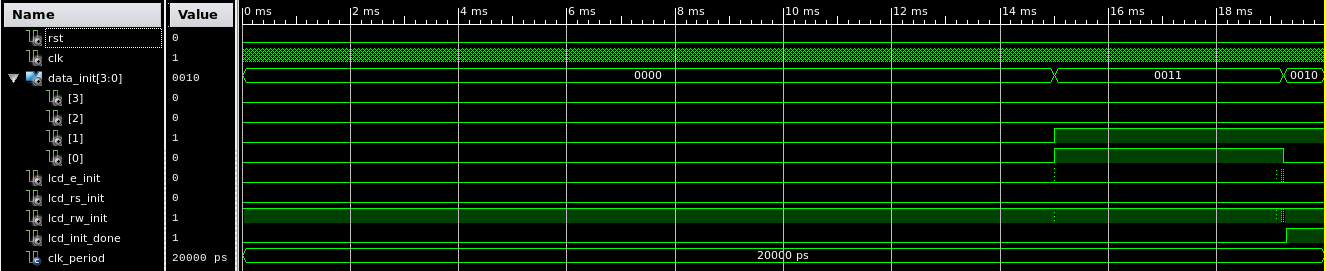
\includegraphics[width=\linewidth]{images/sim_init_geral.png}
    \caption{Forma de onda completa do \textit{testbench} \texttt{lcd\_init\_tb}
             (0 a 20\,ms): quatro pulsos de \texttt{LCD\_E\_INIT} e transição de
             \texttt{LCD\_INIT\_DONE} para '1' ao final da sequência.}
    \label{fig:sim_init_geral}
\end{figure}

A Figura~\ref{fig:sim_init_enable} apresenta uma visão ampliada de um dos pulsos de
\textit{enable}, confirmando a largura de 240\,ns (12 ciclos) com o dado estável em
\texttt{DATA\_INIT = 0x3} e \texttt{LCD\_RW\_INIT = '0'} durante a operação de escrita.

\begin{figure}[H]
    \centering
    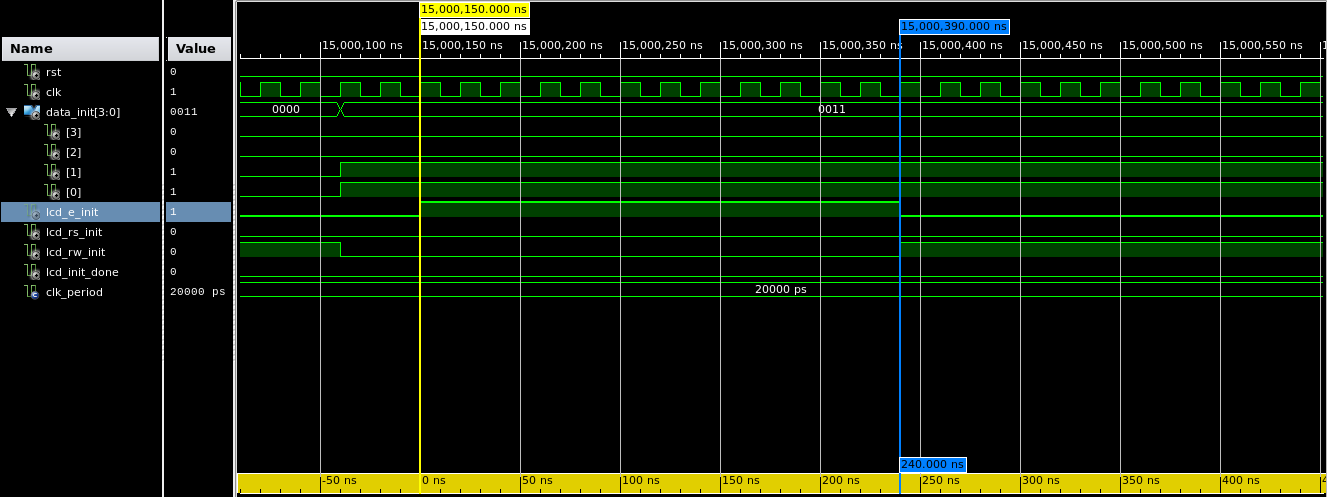
\includegraphics[width=\linewidth]{images/sim_init_enable.png}
    \caption{Detalhe de um pulso de \textit{enable} na inicialização:
             \texttt{DATA\_INIT = 0x3}, pulso de \texttt{LCD\_E\_INIT} com duração
             de 240\,ns (12 ciclos de 20\,ns).}
    \label{fig:sim_init_enable}
\end{figure}

\subsubsection{\textit{Testbench} de Escrita (\texttt{lcd\_write\_tb.vhd})}

O estímulo aplica reset por 100\,ns, libera o reset e, 40\,ns depois, força
\texttt{LCD\_INIT\_DONE = '1'} diretamente, dispensando a necessidade de simular o
módulo de inicialização. A simulação cobre 3{,}2\,ms — tempo suficiente para enviar
os quatro comandos de configuração e os 32 caracteres das duas linhas. A
Figura~\ref{fig:sim_write} ilustra o padrão de dois nibbles por byte em
\texttt{DATA\_OUT}: primeiro o nibble superior, depois o inferior, cada um flanqueado
por um pulso em \texttt{LCD\_E}. O sinal \texttt{LCD\_RS} distingue comandos
(\texttt{'0'}) de caracteres (\texttt{'1'}).

\begin{figure}[H]
    \centering
    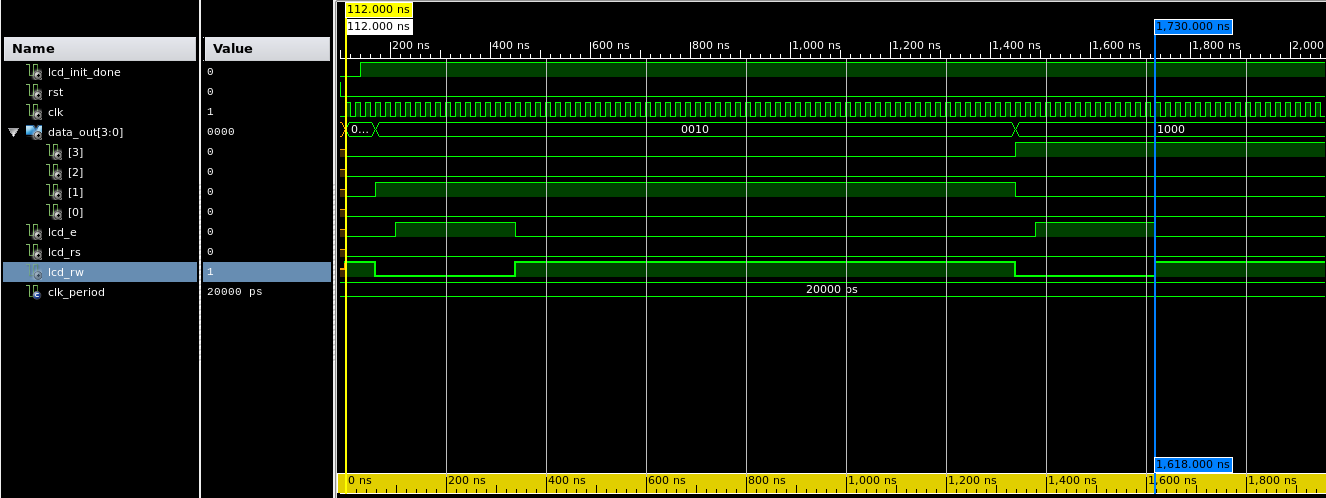
\includegraphics[width=\linewidth]{images/sim_write.png}
    \caption{Forma de onda do \textit{testbench} \texttt{lcd\_write\_tb}: envio dos
             comandos de configuração e dos caracteres em modo 4 bits, com dois
             nibbles por byte visíveis em \texttt{DATA\_OUT}.}
    \label{fig:sim_write}
\end{figure}

\subsubsection{\textit{Testbench} do Módulo de Topo (\texttt{top\_tb.vhd})}

O \textit{testbench} de nível superior integra os dois módulos e simula o fluxo
completo por 23\,ms. A Figura~\ref{fig:sim_top} evidencia a transição entre as fases
de inicialização e escrita no barramento \texttt{SF\_D}: durante a inicialização, o
barramento reflete as saídas de \texttt{lcd\_init}; após \texttt{LCD\_INIT\_DONE}
ir a '1', passa a refletir as saídas de \texttt{lcd\_write}. O sinal \texttt{SF\_CE0}
permanece em '1' durante toda a simulação, confirmando que a Strata Flash está
continuamente desabilitada.

\begin{figure}[H]
    \centering
    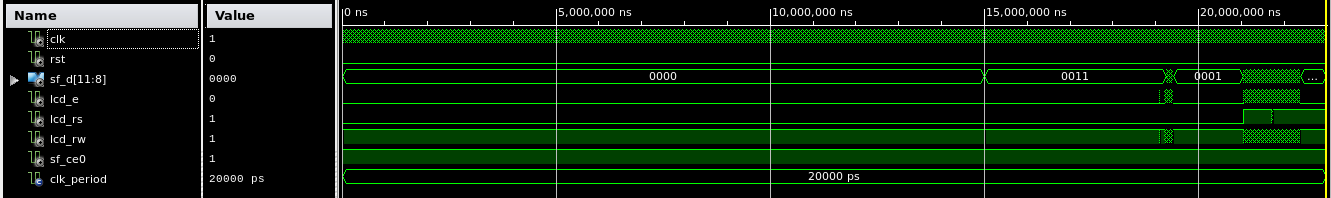
\includegraphics[width=\linewidth]{images/sim_top.png}
    \caption{Forma de onda do \textit{testbench} \texttt{top\_tb} (0 a 23\,ms):
             integração dos módulos de inicialização e escrita, com transição de
             \texttt{SF\_D} após \texttt{LCD\_INIT\_DONE} e \texttt{SF\_CE0}
             permanentemente em '1'.}
    \label{fig:sim_top}
\end{figure}

% ==============================================================
\subsection{Exercício 3 – Implementação e Teste na Placa}
% ==============================================================

\question{Faça a síntese, implementação e geração do arquivo \texttt{.bit}. Programe
a placa e teste o comportamento do LCD com a mensagem definida pelo grupo.}

\answer
O projeto foi sintetizado e implementado no Xilinx ISE Project Navigator para a FPGA
Spartan-3E (XC3S500E) da placa Digilent Nexys~2. O arquivo de restrições
\texttt{top.ucf} define as seguintes atribuições de pinos:

\begin{itemize}
    \item \textbf{CLK} $\rightarrow$ C9: oscilador de 50\,MHz da placa
          (padrão LVCMOS33).
    \item \textbf{RST} $\rightarrow$ K17: botão com resistor de \textit{pull-down}
          integrado (padrão LVTTL, lógica positiva).
    \item \textbf{LCD\_E} $\rightarrow$ M18, \textbf{LCD\_RS} $\rightarrow$ L18,
          \textbf{LCD\_RW} $\rightarrow$ L17: sinais de controle do LCD (LVCMOS33,
          4\,mA, \textit{slew} lento).
    \item \textbf{SF\_D[11:8]} $\rightarrow$ R15, R16, P17, M15: barramento de dados
          DB7–DB4 do LCD (LVCMOS33, 4\,mA, \textit{slew} lento).
    \item \textbf{SF\_CE0} $\rightarrow$ D16: \textit{chip enable} da Strata Flash,
          mantido em '1' (LVCMOS33, 4\,mA, \textit{slew} lento).
\end{itemize}

Após a geração do arquivo \texttt{.bit} e a programação da placa via cabo JTAG, o
display LCD exibiu corretamente a mensagem nas duas linhas:

\begin{center}
    \texttt{Durma bem}\\
    \texttt{cedo, OK?}
\end{center}

O funcionamento completo na placa pode ser verificado no vídeo disponível em:
\begin{center}
    \url{https://youtu.be/TAssUaDmJUQ?si=uqXNVINxnoEmbtkE}
\end{center}

\end{document}